\begin{myblock}{{\large Introduction}}
	
\textbf{Motivation:}\\
 the Search and Rescue Robots Market is projected to grow with a Compound Annual Growth Rate (CAGR) of more than 20\%\footnote{\url{https://www.mordorintelligence.com/industry-reports/search-and-rescue-robots-market}}.
 Allied Market Research, reported that the global inspection, and surveillance robots market generated \$940 million in 2020 and is expected to reach close to \$14 billion by 2030\footnote{\url{https://www.cnbc.com/2021/12/26/robotic-dogs-taking-on-jobs-in-security-inspection-and-public-safety-.html}}.	\\
%
\textbf{Problem:}\\
\begin{itemize}
	\setlength{\itemindent}{-10pt}
	\item lack of \textit{generic} and \textit{robot agnostic} control software solutions to control quadruped robots,
	\item high level of expertise required to control such platforms,
	\item increased complexity when the quadruped robots are equipped with one (or more) manipulator(s).
\end{itemize}
\vspace{20pt}
	
\textbf{Solution:} Wolf
\begin{figure}[thb!]
	\centering
	
\includegraphics[width=0.5\columnwidth, trim={7cm 5.5cm 7cm 5.5cm}, clip=true]{images/wolf-logo.pdf}
	\label{fig:wolf_logo}
\end{figure}

\vspace{20pt}
\textbf{In detail:}\\
\begin{itemize}
	\setlength{\itemindent}{-10pt}
	\item WoLF is an end-to-end software suite devoted to the loco-manipulation of quadruped robots,
	\item it abstracts the complexity of planning and control of quadrupedal robot hardware,
	\item it allows multiple tele-operation devices attached to the robot.
	\end{itemize}
\end{myblock} 

\begin{myblock}{\large How it started} 
%
The WoLF project started from the work in~\cite{raiola2020} about a novel locomotion framework for quadrupedal robots. 
We designed it to work as a plugin for ros\_control \cite{chitta2017ros_control}. The ros\_control package permits to easily abstract the particular hardware for both the quadruped and/or the manipulator and therefore to re-use the same controller with different robots provided that they expose an effort interface.
%
\end{myblock}

\begin{myblock}{\large Components} 
%
\begin{figure}
	\centering
	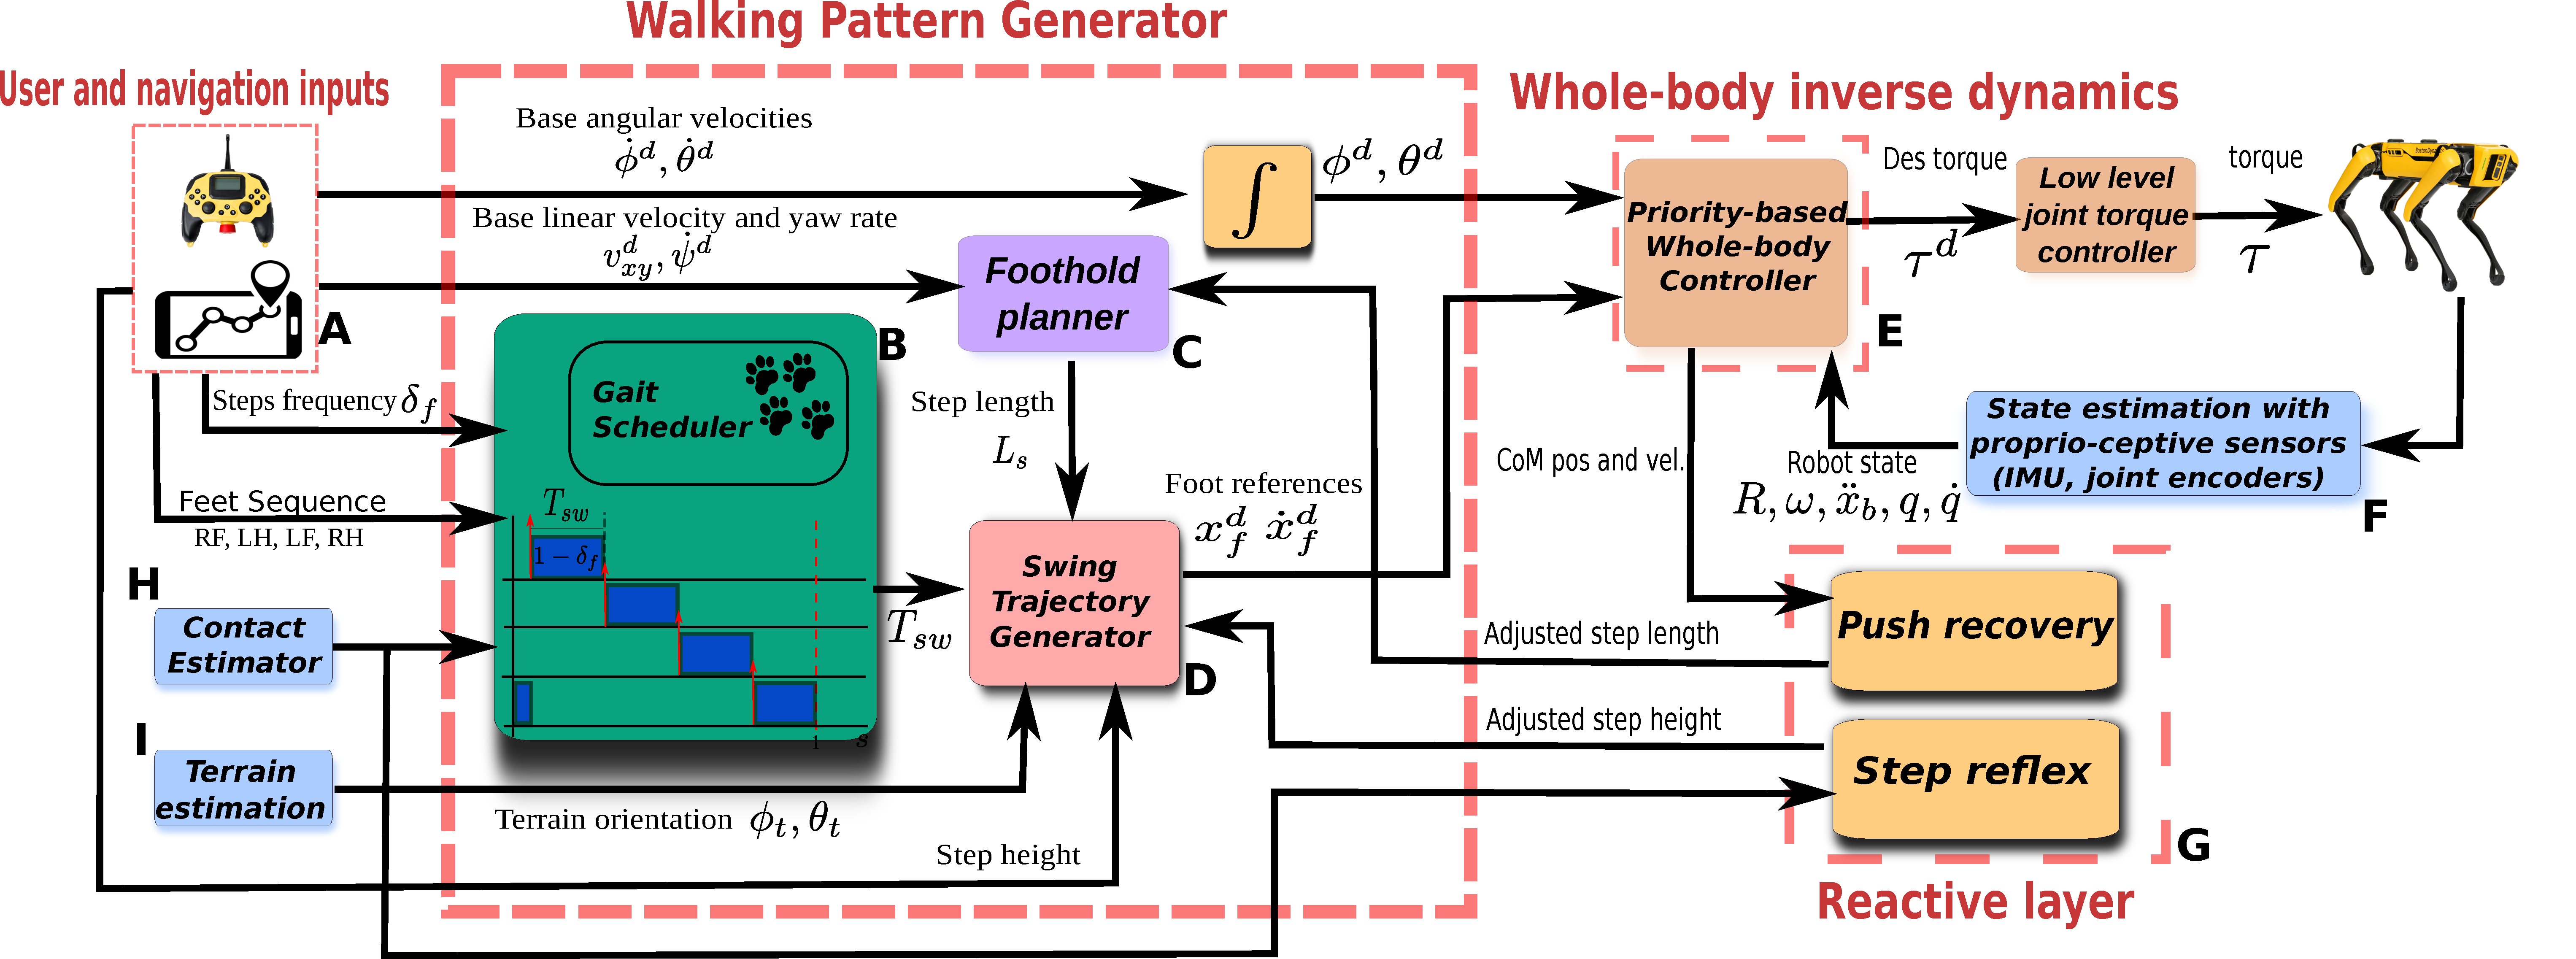
\includegraphics[width=\textwidth]{images/block_diagram_updated.pdf}
	\caption{WoLF block diagram overview.}
	\label{fig:diagram}
\end{figure}
\begin{enumerate}[label=\Alph*]
	\item the \emph{user interface} provides control of the robot through multiple devices (joy-pads, keyboards, GUI, ROS topics and services, etc...),
	\item a \emph{gait scheduler} coordinates the footsteps based on the gait schedule,
	\item the \emph{foothold planner} transforms base twist commands into footholds,
	\item the \emph{swing trajectory generator} calculates the swing trajectory for the feet based on the desired footholds and the estimated terrain slope,
	\item a \emph{whole-body inverse dynamics layer} is in charge to track user/navigation inputs and walking pattern generator references and transforming them into torque commands,
	\item the \emph{state estimation} uses proprioceptive sensors and IMU to compute the actual twist of the robot's floating-base,
	\item the \emph{reactive layer} provides push recovery and step reflex capabilities,
	\item the \emph{contact estimation} module provides the status of the foot contacts throught the joint torque sensors, or through contact sensors if these are available in the platform,
	\item the \emph{terrain estimation} estimates the terrain plane over the feet at stance and re-orients the friction cones and the swing trajectories such that the robot can climb up ramps and stairs \cite{focchi2020heuristic} without scuffing.
\end{enumerate}
\end{myblock}

%\begin{myblock}{\large Wolf components}
%
%\textbf{Features:}
%\begin{itemize}
%	\item plug-and-play software framework easy to tune and adaptable to any quadruped robot without the need for specific knowledge about locomotion or control,
%	\item promote strandardization: use of established robotics tools and technologies such as ROS~\cite{quigley2009ros}, Gazebo~\cite{agueroVRC2015}, OpenSoT~\cite{hoffmanOpenSoT2017},
%	\item extend the capabilities of quadrupedal platforms with manipulation and navigation skills.
%\end{itemize}
%
%\textbf{How is it done?}\\
%\vspace{20pt}
%The WoLF project started from the work in~\cite{raiola2020} about a novel locomotion framework for quadrupedal robots. 
%We designed it to work as a plugin for ros\_control \cite{chitta2017ros_control}. The ros\_control package permits to easily abstract the particular hardware for both the quadruped and/or the manipulator and therefore to re-use the same controller with different robots provided that they expose an effort interface.
%\end{myblock}

%\begin{myblock}{\large Wolf components}
	
	%\begin{columns}
	%\begin{column}{0.63\textwidth}
	
%	\textbf{How is it done?}\\
%	\begin{itemize}
%		\item User inputs and navigation
%		\item Walking pattern generator and reactive layer
%		\item State and Terrain Estimation
%		\item Whole-Body Inverse Dynamics
%	\end{itemize}
	%\end{column}
	%\begin{column}{0.3\textwidth}
	%\begin{figure}[tb]
	%	\centering
	%	\includegraphics[width=0.9\columnwidth]{figures/model.pdf}
	%\end{figure}
	%\end{column}	
	%\end{columns}	
%\end{myblock}
